% !TEX TS-program = pdflatex
% !TEX encoding = UTF-8 Unicode

% This is a simple template for a LaTeX document using the "article" class.
% See "book", "report", "letter" for other types of document.

\documentclass[11pt]{article} % use larger type; default would be 10pt

\usepackage[utf8]{inputenc} % set input encoding (not needed with XeLaTeX)

%%% Examples of Article customizations
% These packages are optional, depending whether you want the features they provide.
% See the LaTeX Companion or other references for full information.

%%% PAGE DIMENSIONS
\usepackage{geometry} % to change the page dimensions
\geometry{a4paper} % or letterpaper (US) or a5paper or....
% \geometry{margin=2in} % for example, change the margins to 2 inches all round
% \geometry{landscape} % set up the page for landscape
%   read geometry.pdf for detailed page layout information

\usepackage{graphicx} % support the \includegraphics command and options

% \usepackage[parfill]{parskip} % Activate to begin paragraphs with an empty line rather than an indent

%%% PACKAGES
\usepackage{booktabs} % for much better looking tables
\usepackage{array} % for better arrays (eg matrices) in maths
\usepackage{paralist} % very flexible & customisable lists (eg. enumerate/itemize, etc.)
\usepackage{verbatim} % adds environment for commenting out blocks of text & for better verbatim
\usepackage{subfig} % make it possible to include more than one captioned figure/table in a single float
\usepackage{graphicx} % includes image inserting into PDFs 
\usepackage[dvipsnames]{xcolor}
\usepackage{fancyvrb}
% These packages are all incorporated in the memoir class to one degree or another...

%%% HEADERS & FOOTERS
\usepackage{fancyhdr} % This should be set AFTER setting up the page geometry
\pagestyle{fancy} % options: empty , plain , fancy
\renewcommand{\headrulewidth}{0pt} % customise the layout...
\lhead{}\chead{}\rhead{}
\lfoot{}\cfoot{\thepage}\rfoot{}

%%% SECTION TITLE APPEARANCE
\usepackage{sectsty}
\allsectionsfont{\sffamily\mdseries\upshape} % (See the fntguide.pdf for font help)
% (This matches ConTeXt defaults)

%%% ToC (table of contents) APPEARANCE
\usepackage[nottoc,notlof,notlot]{tocbibind} % Put the bibliography in the ToC
\usepackage[titles,subfigure]{tocloft} % Alter the style of the Table of Contents
\renewcommand{\cftsecfont}{\rmfamily\mdseries\upshape}
\renewcommand{\cftsecpagefont}{\rmfamily\mdseries\upshape} % No bold!


%%%Matlab Code Requirements
\usepackage{listings}
\usepackage{color} %red, green, blue, yellow, cyan, magenta, black, white
\definecolor{mygreen}{RGB}{28,172,0} % color values Red, Green, Blue
\definecolor{mylilas}{RGB}{170,55,241}
\graphicspath{ {images/} }
%%% END Article customizations

%%% The "real" document content comes below...

\title{Homework 5}
\author{Prithviraj Kadiyala}
%\date{} % Activate to display a given date or no date (if empty),
         % otherwise the current date is printed 

\begin{document}
\maketitle

\section{First Answer or 1a}

% redefine \VerbatimInput
\RecustomVerbatimCommand{\VerbatimInput}{VerbatimInput}%
{fontsize=\footnotesize,
 %
 frame=lines,  % top and bottom rule only
 framesep=2em, % separation between frame and text
 rulecolor=\color{Gray},
 %
 label=\fbox{\color{Black}Results},
 labelposition=topline,
 %
 commandchars=\|\(\), % escape character and argument delimiters for
                      % commands within the verbatim
 commentchar=*        % comment character
}


\lstset{language=Matlab,%
    %basicstyle=\color{red},
    breaklines=true,%
    morekeywords={matlab2tikz},
    keywordstyle=\color{blue},%
    morekeywords=[2]{1}, keywordstyle=[2]{\color{black}},
    identifierstyle=\color{black},%
    stringstyle=\color{mylilas},
    commentstyle=\color{mygreen},%
    showstringspaces=false,%without this there will be a symbol in the places where there is a space
    numbers=left,%
    numberstyle={\tiny \color{black}},% size of the numbers
    numbersep=9pt, % this defines how far the numbers are from the text
    emph=[1]{for,end,break},emphstyle=[1]\color{red}, %some words to emphasise
    %emph=[2]{word1,word2}, emphstyle=[2]{style},    
}
\subsection*{Matlab Code}
\lstinputlisting{HW5_1a.m}
Output Images:
\begin{figure}
 \centering
	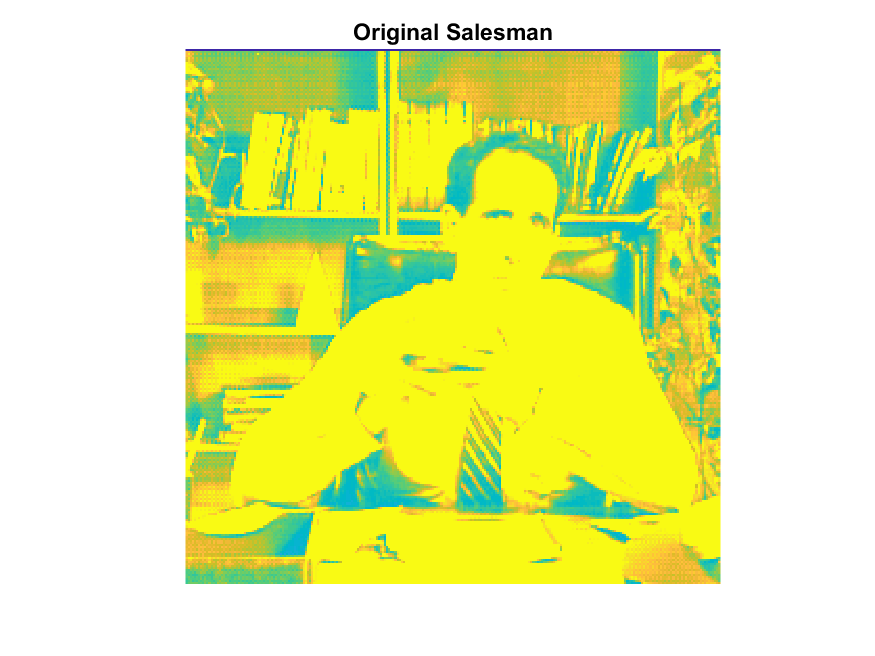
\includegraphics{1aa.png}
	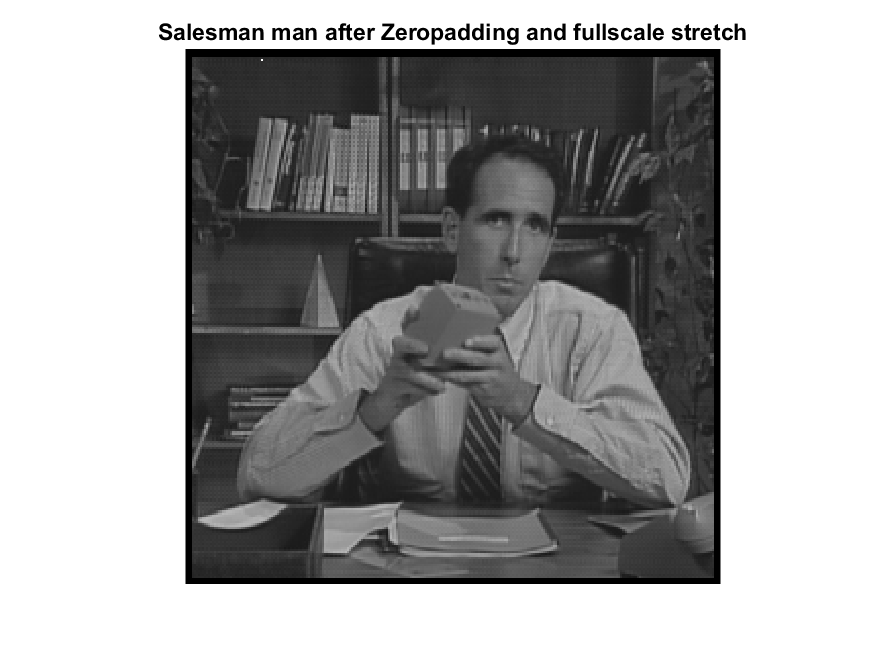
\includegraphics{1ab.png}
\end{figure}
\begin{figure}
\centering
	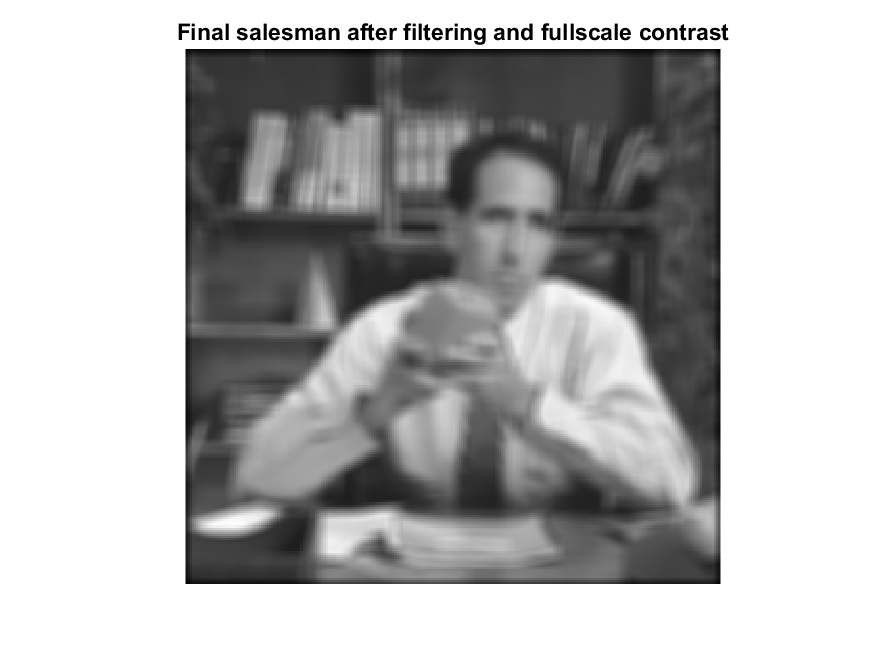
\includegraphics{1ac.png}
\end{figure}
\clearpage

\section {Second Answer or 1b}
\subsection*{Matlab Code}
\lstinputlisting{HW5_1b.m}
Output Images: 
\begin{figure}
 \centering
	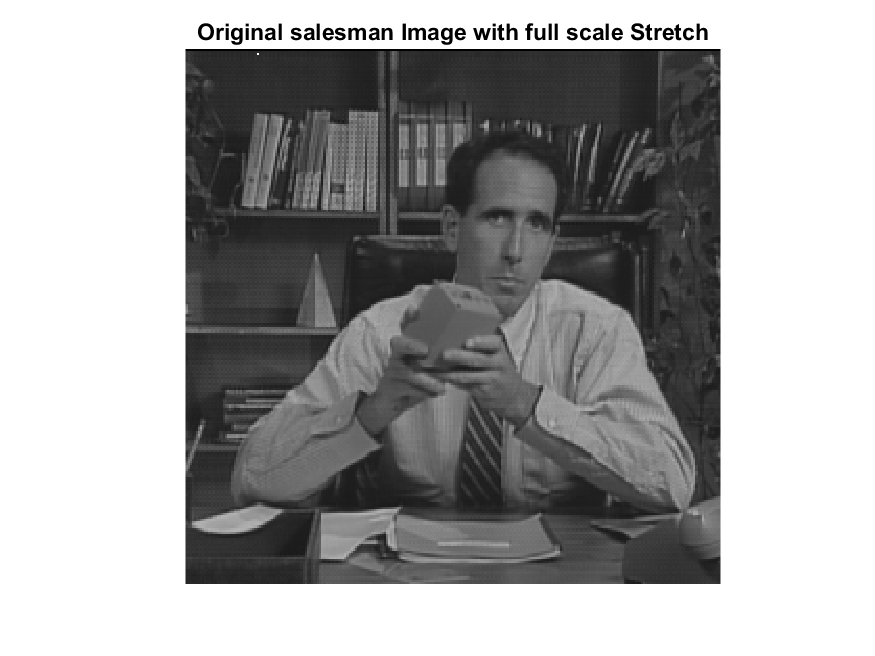
\includegraphics{1ba.png}
	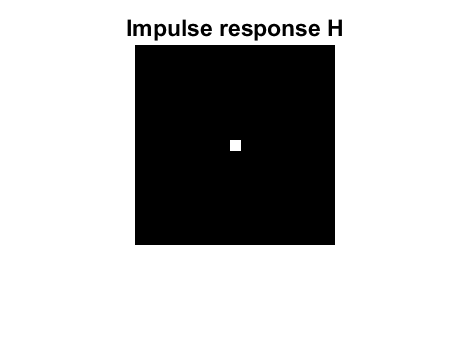
\includegraphics{1bb.png}
\end{figure}
\begin{figure}
\centering
	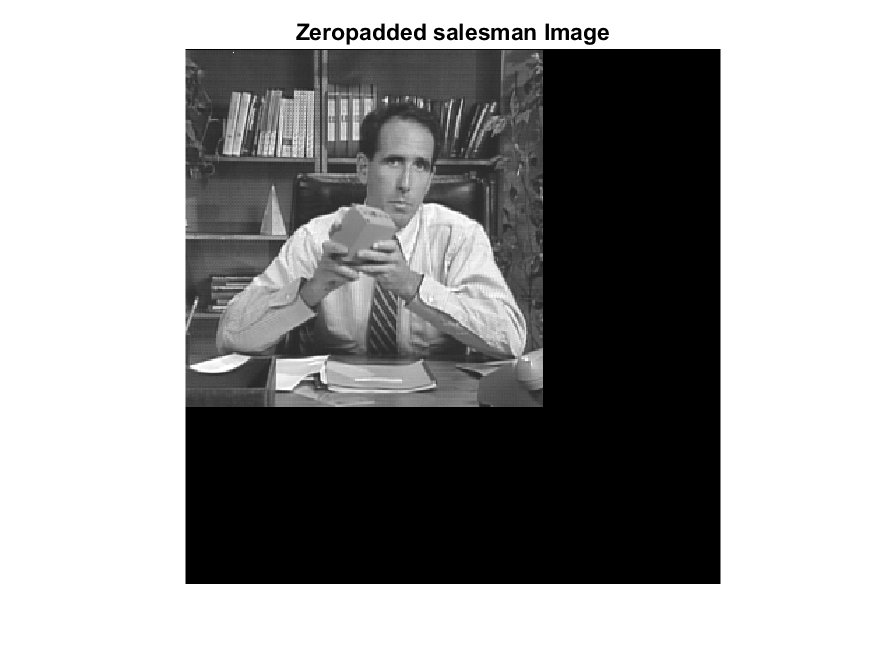
\includegraphics{1bc.png}
	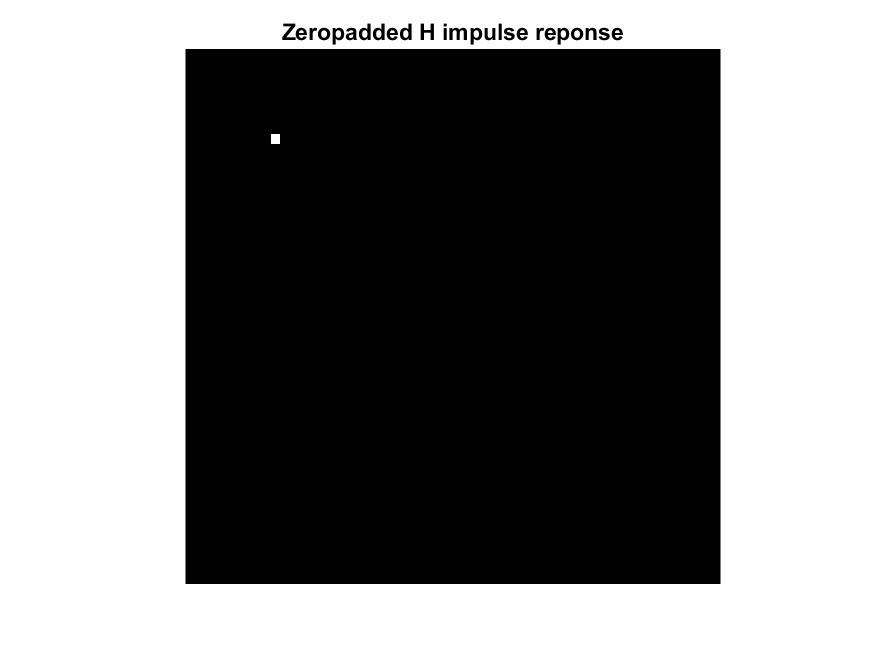
\includegraphics{1bd.png}
\end{figure}
\begin{figure}
\centering
	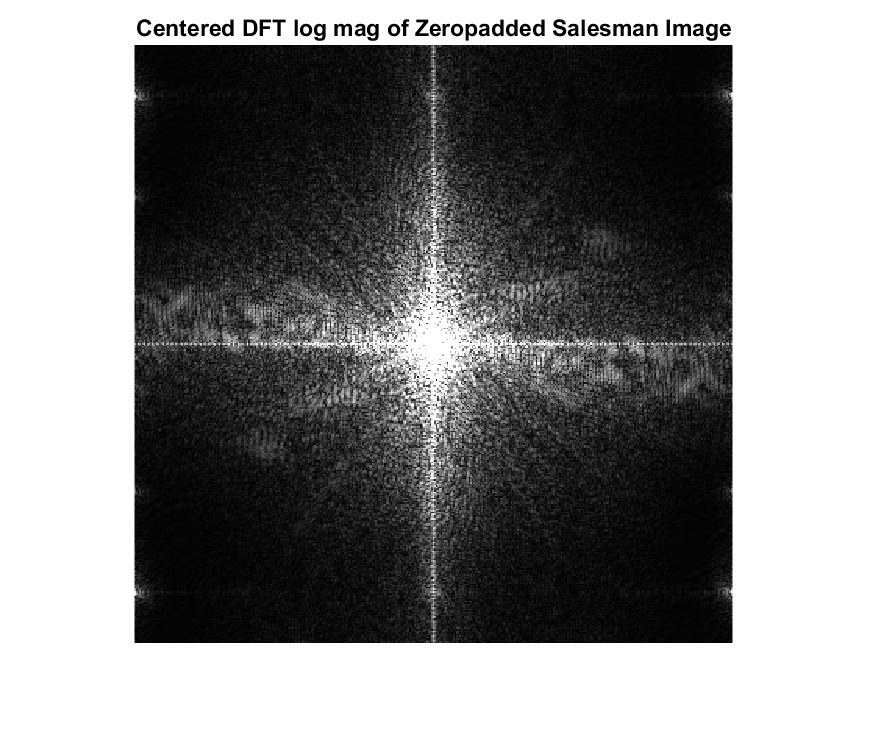
\includegraphics{1be.png}
	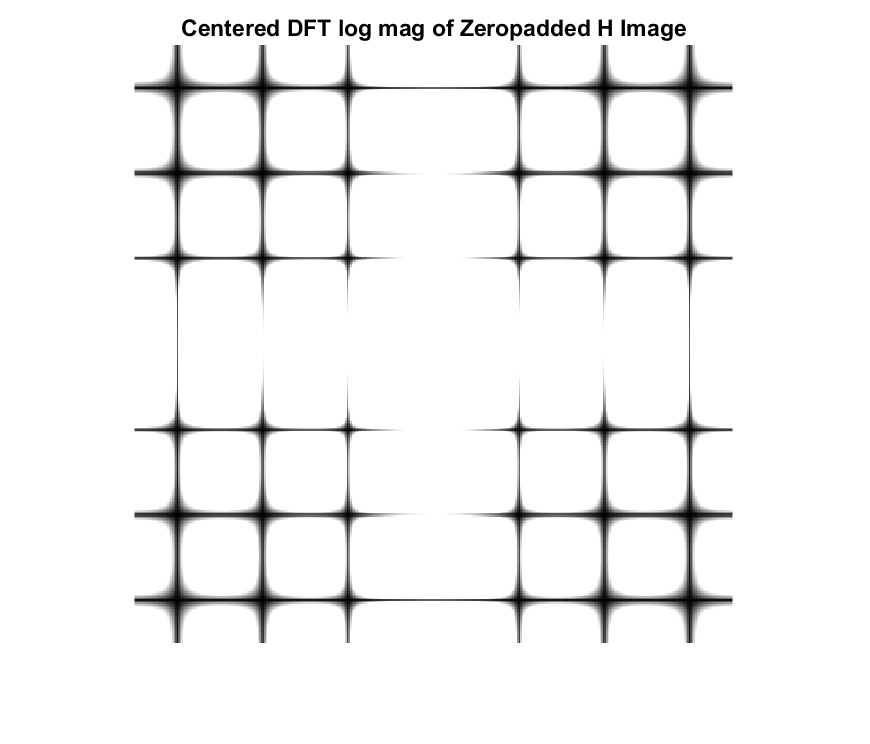
\includegraphics{1bf.png}
\end{figure}
\begin{figure}
\centering
	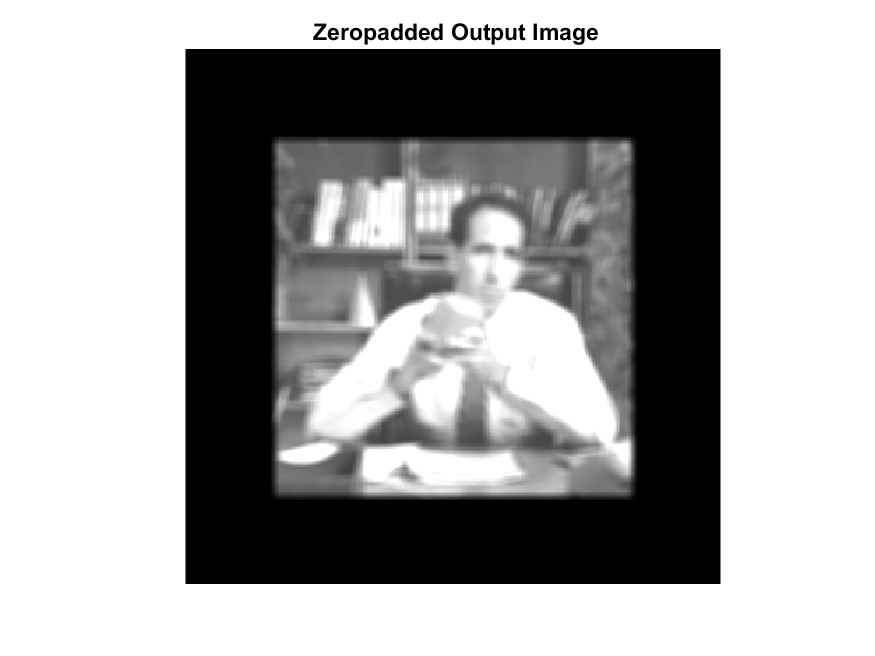
\includegraphics{1bg.png}
	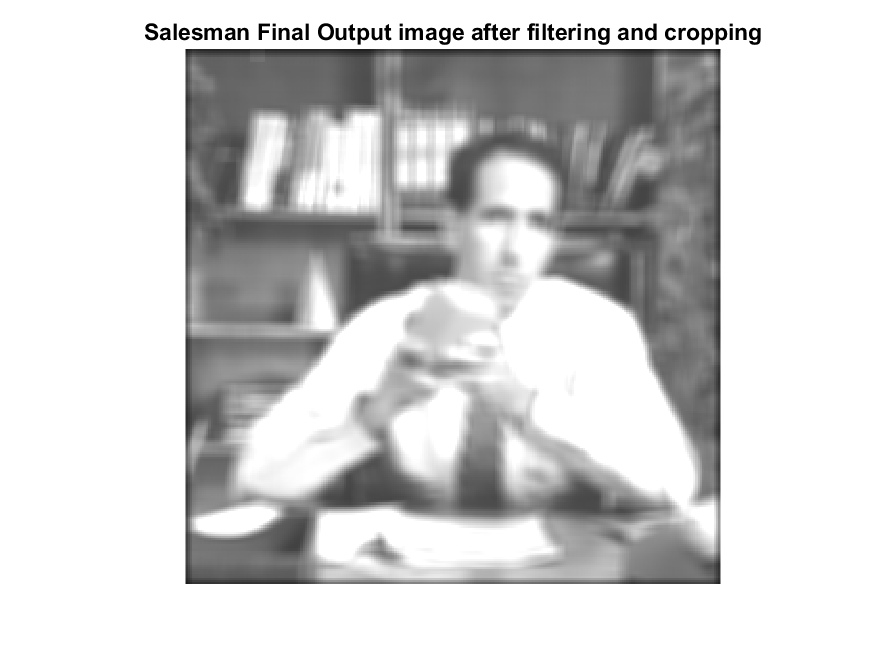
\includegraphics{1bh.png}
\end{figure}
\clearpage

\section {Third Answer or 1c}
\subsection*{Matlab Code}
\lstinputlisting{HW5_1c.m}
Output Images: 
\begin{figure}
 \centering
	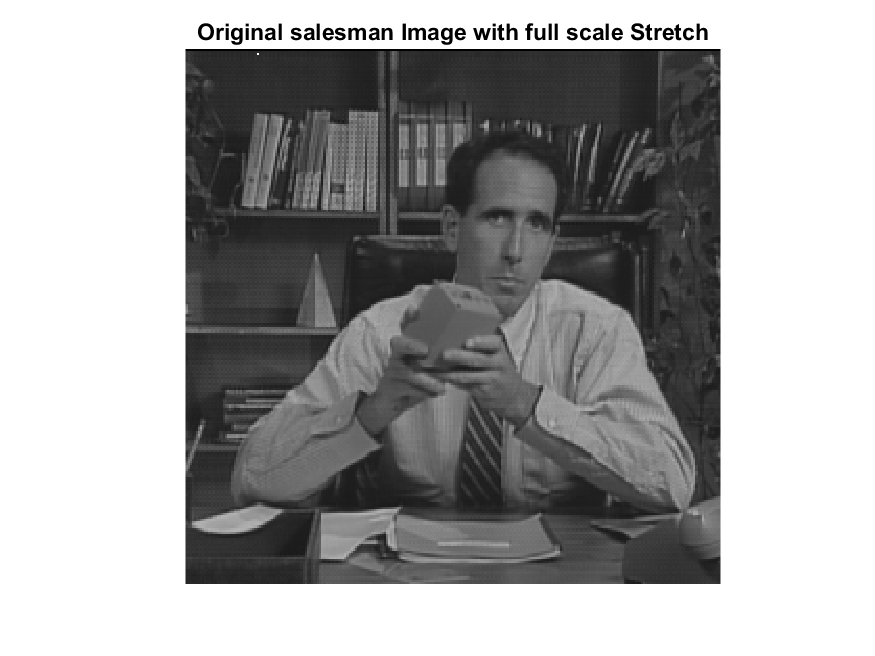
\includegraphics{1ca.png}
	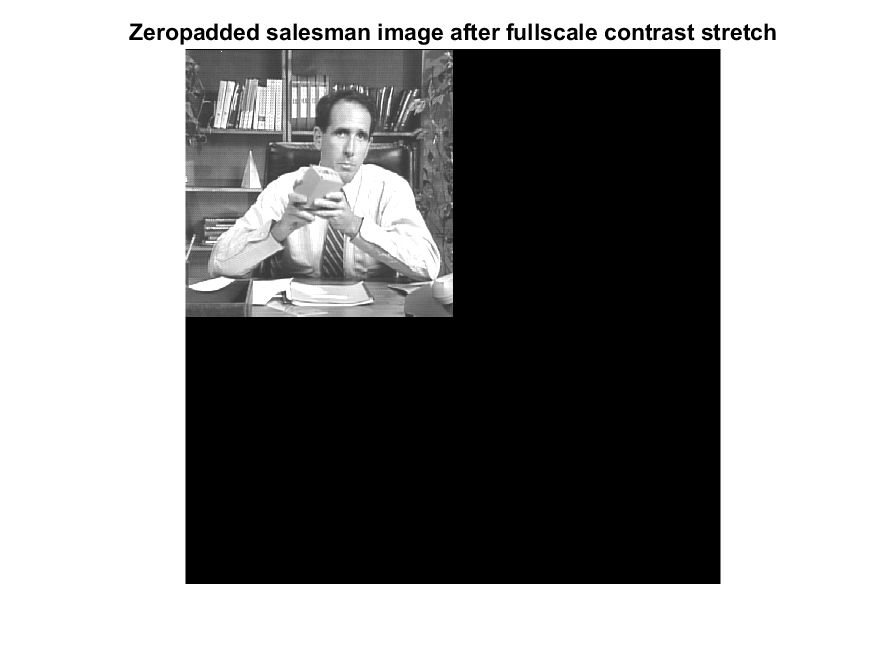
\includegraphics{1cb.png}
\end{figure}
\begin{figure}
 \centering
	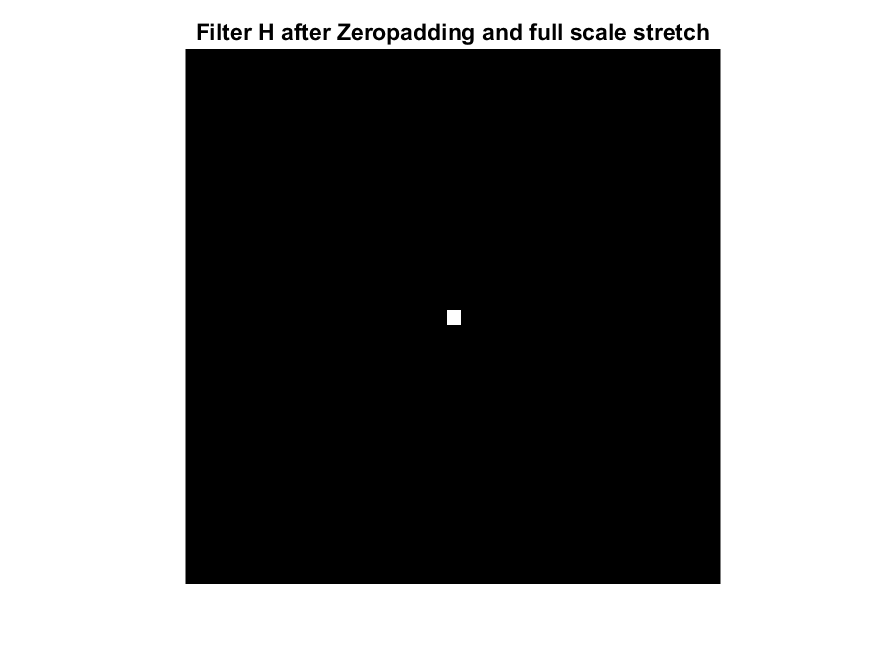
\includegraphics{1cc.png}
	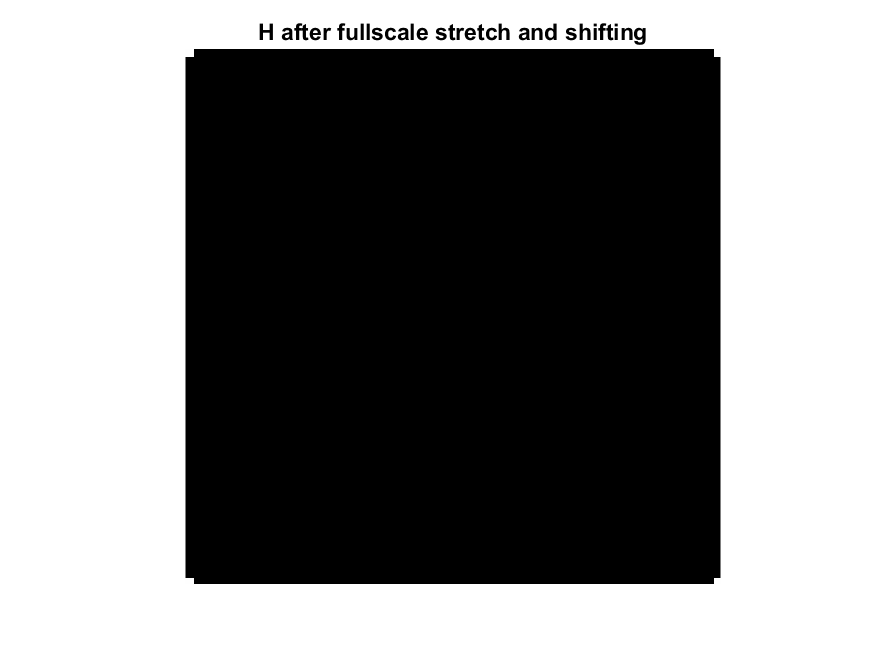
\includegraphics{1cd.png}
\end{figure}
\begin{figure}
 \centering
	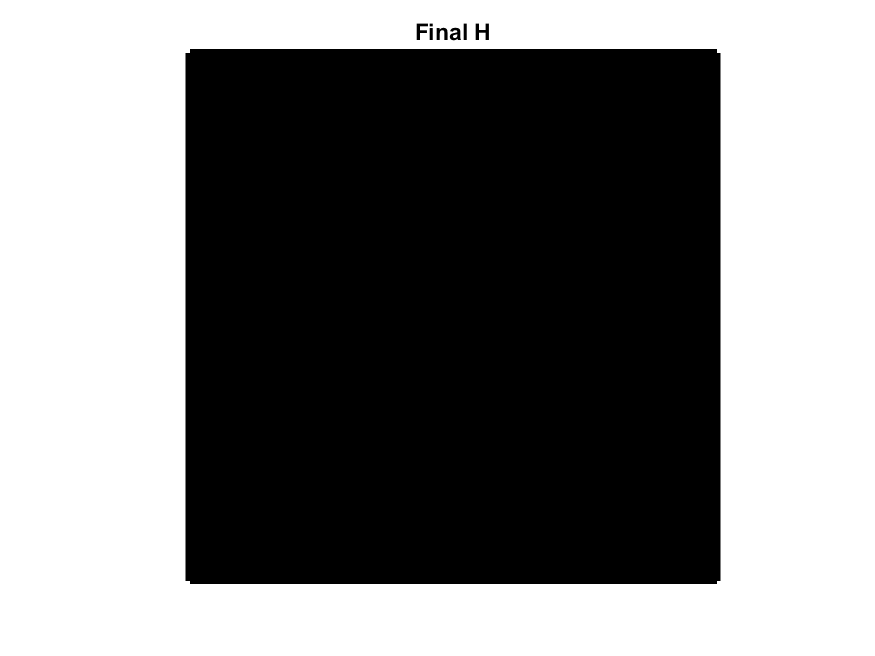
\includegraphics{1ce.png}
	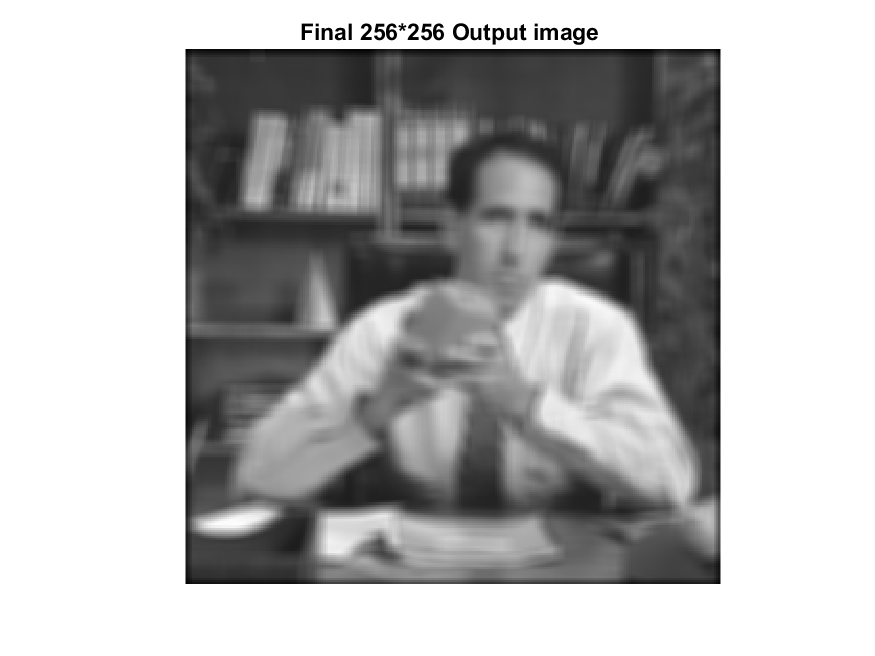
\includegraphics{1cf.png}
\end{figure}
\clearpage

\section {Fourth Answer or 2a}
\subsection*{Matlab Code}
\lstinputlisting{HW5_2a.m}

Output:
\VerbatimInput{Q2a.txt}

Output Images: 
\begin{figure}
 \centering
	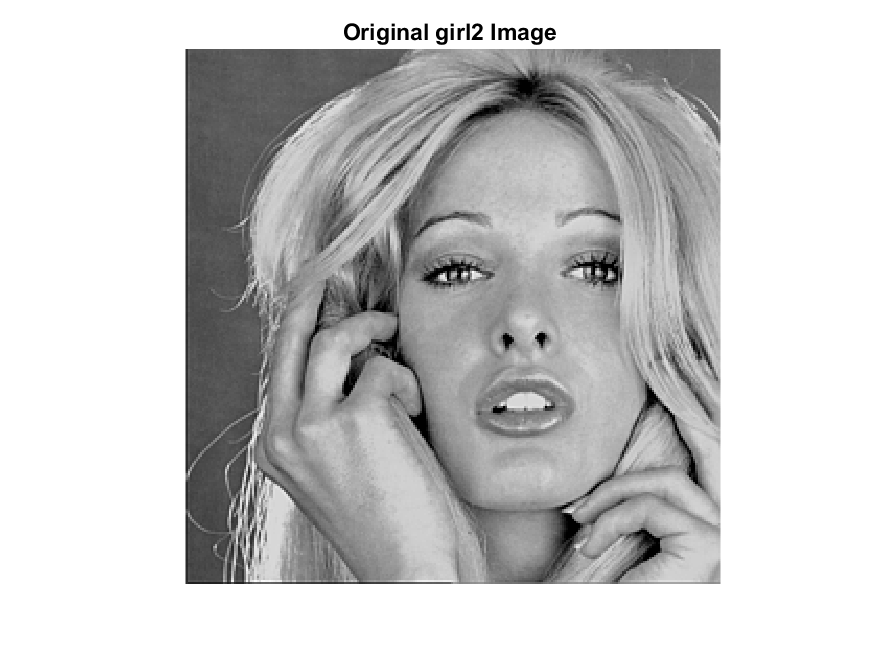
\includegraphics{2aa.png}
	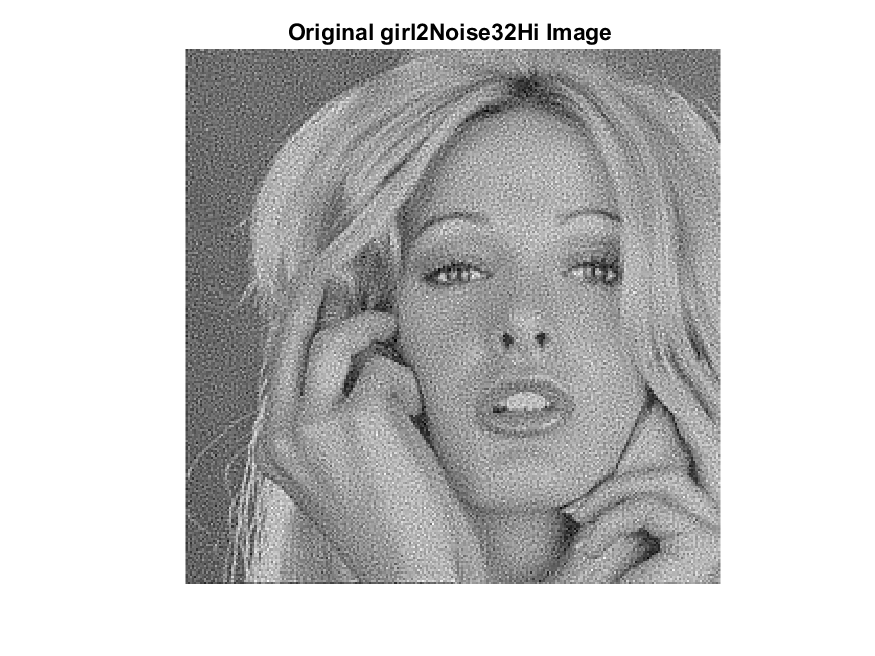
\includegraphics{2ab.png}
\end{figure}
\begin{figure}
 \centering
	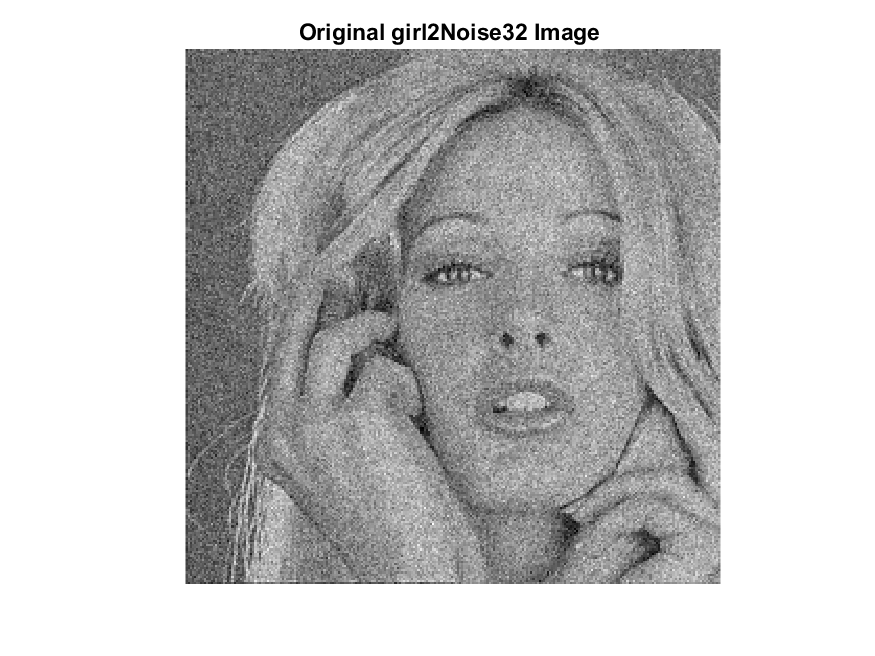
\includegraphics{2ac.png}
\end{figure}
\clearpage

\section {Fifth Answer or 2b}
\subsection*{Matlab Code}
\lstinputlisting{HW5_2b.m}

Output:
\VerbatimInput{Q2b.txt}


Output Images: 
\begin{figure}
 \centering
	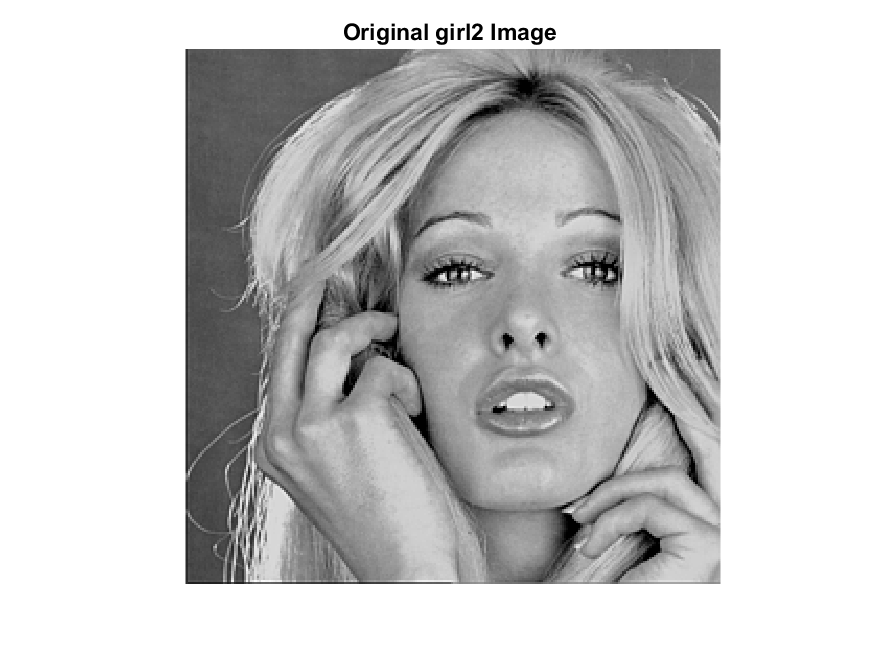
\includegraphics{2ba.png}
	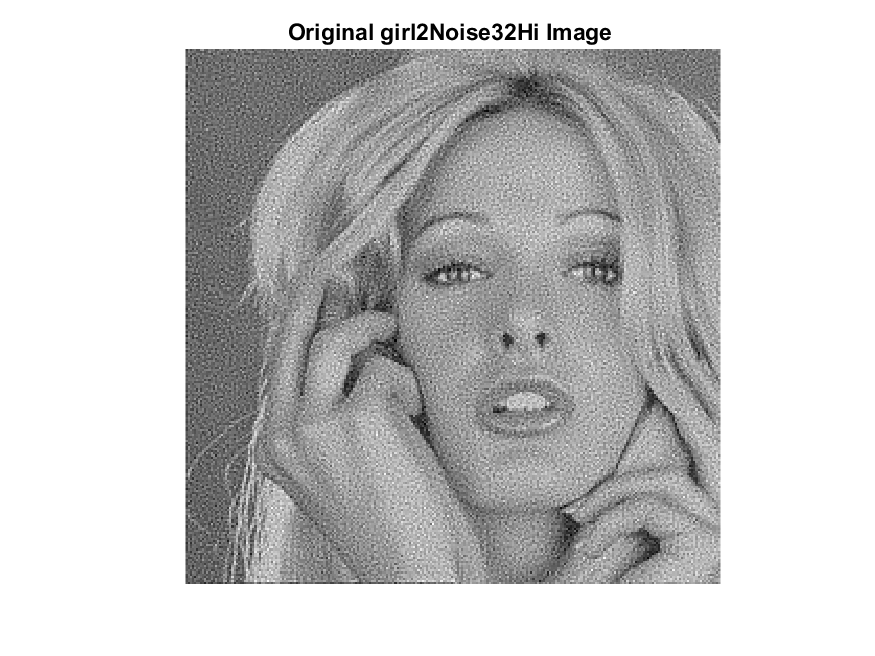
\includegraphics{2bb.png}
\end{figure}
\begin{figure}
 \centering
	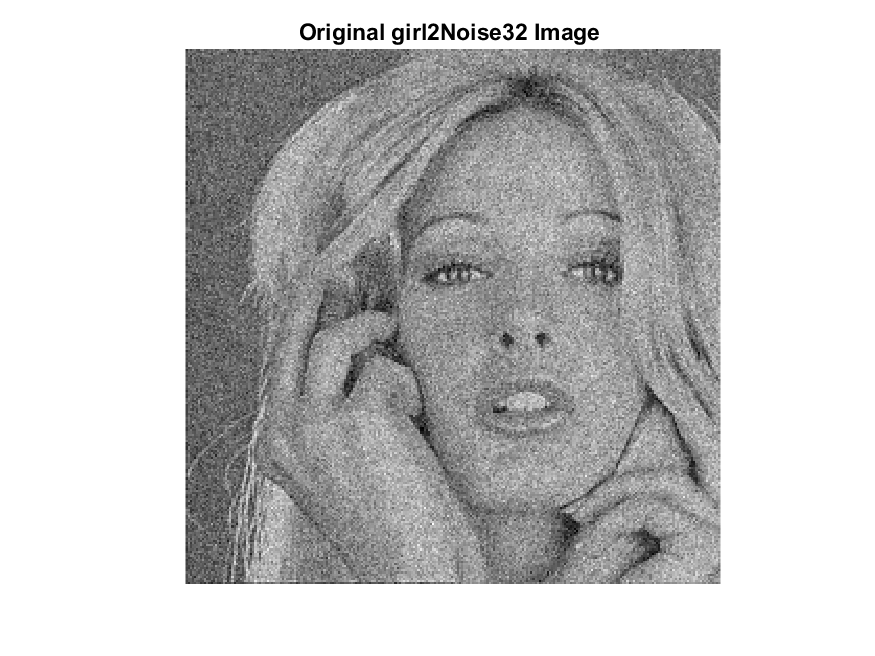
\includegraphics{2bc.png}
	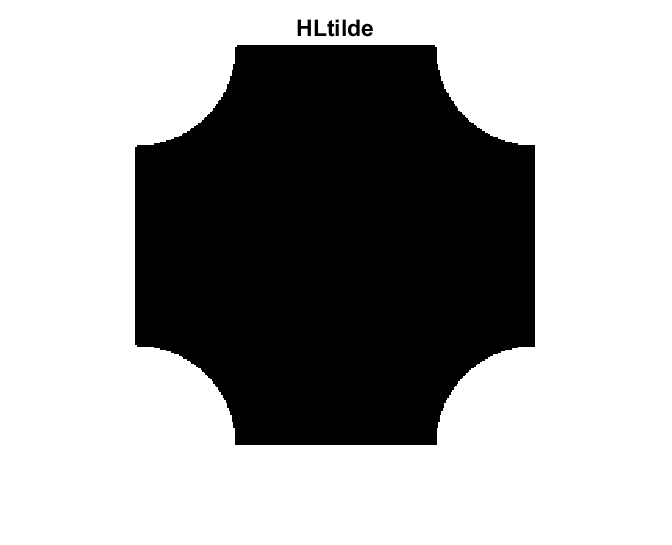
\includegraphics{2bd.png}
\end{figure}
\begin{figure}
 \centering
	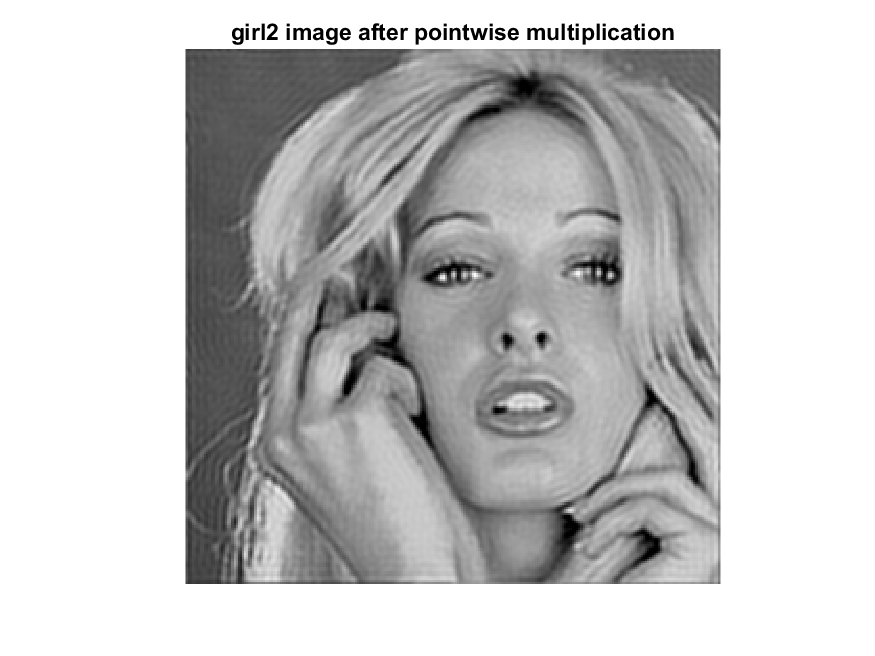
\includegraphics{2be.png}
	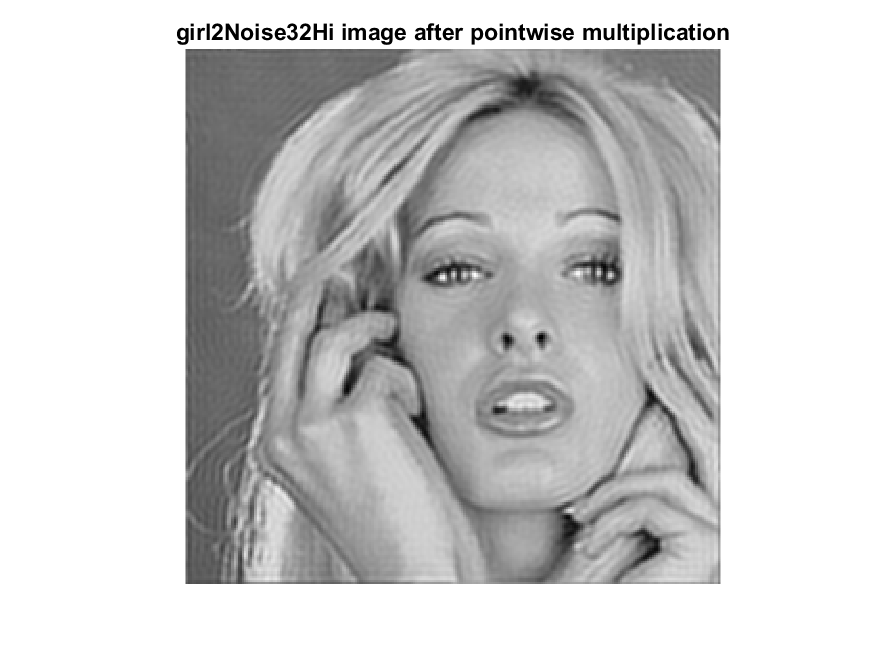
\includegraphics{2bf.png}
\end{figure}
\begin{figure}
 \centering
	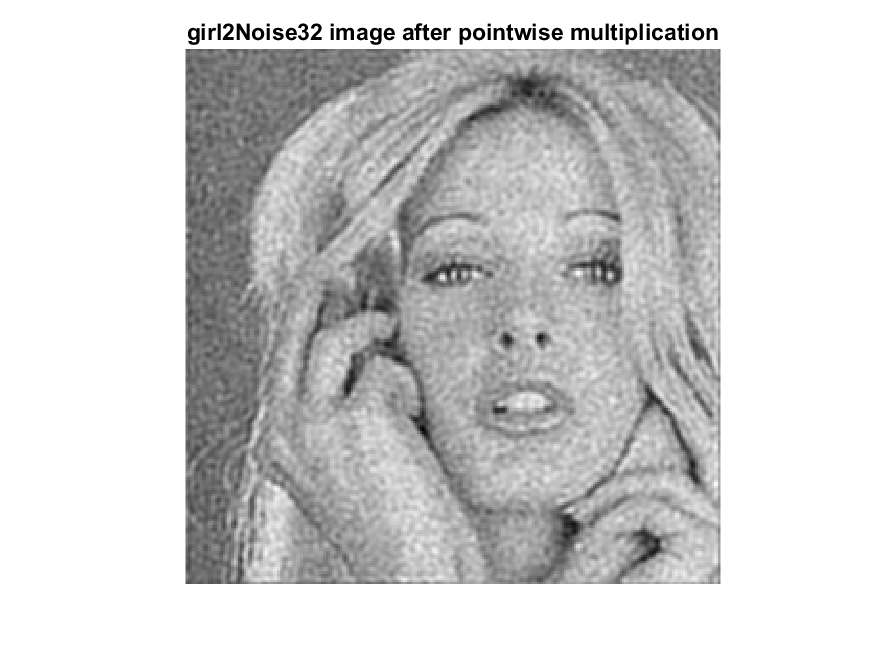
\includegraphics{2bg.png}
\end{figure}
\clearpage 

\section {Sixth Answer or 2c}
\subsection*{Matlab Code}
\lstinputlisting{HW5_2c.m}

Output:
\VerbatimInput{Q2c.txt}


Output Images: 
\begin{figure}
 \centering
	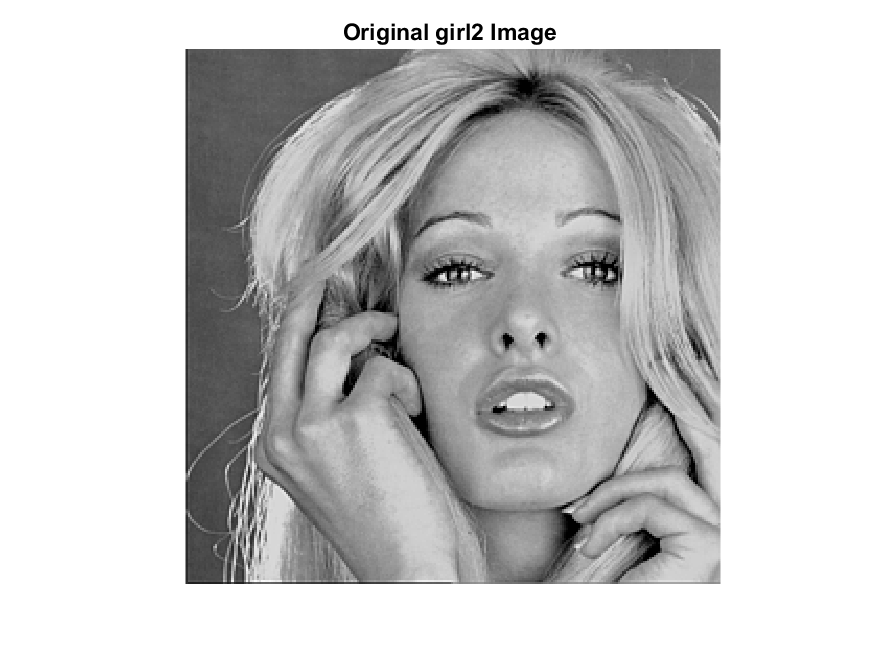
\includegraphics{2ca.png}
	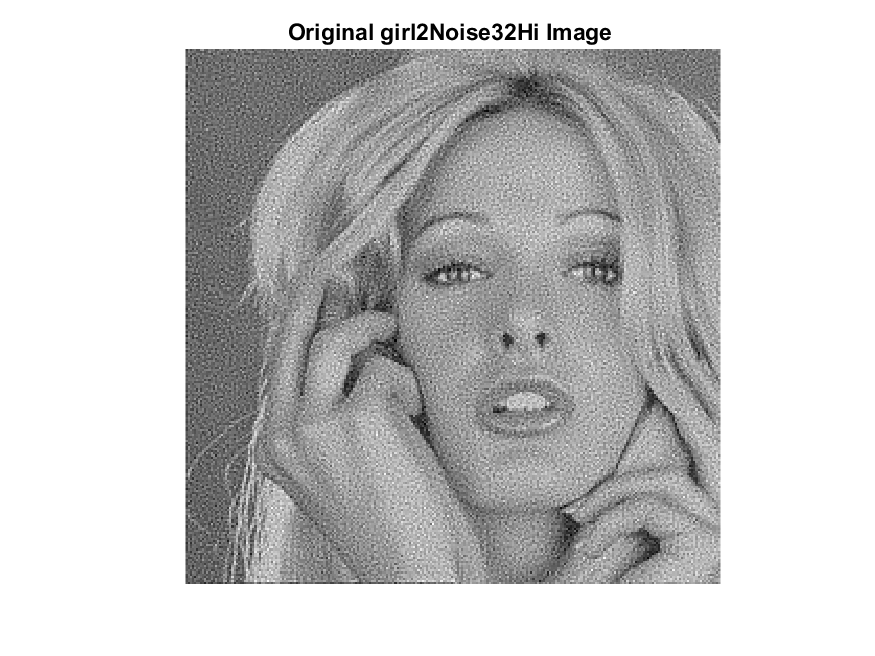
\includegraphics{2cb.png}
\end{figure}
\begin{figure}
 \centering
	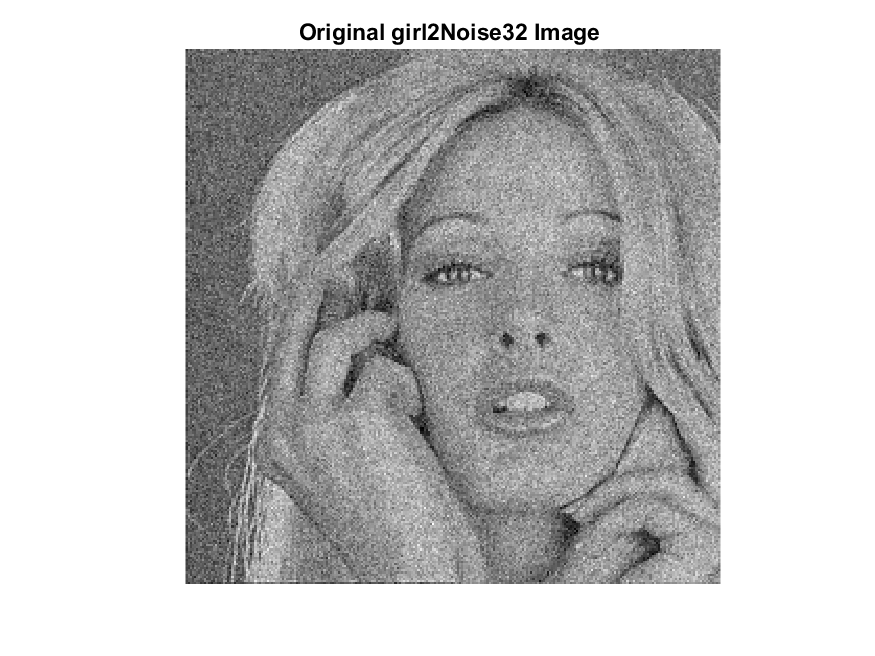
\includegraphics{2cc.png}
	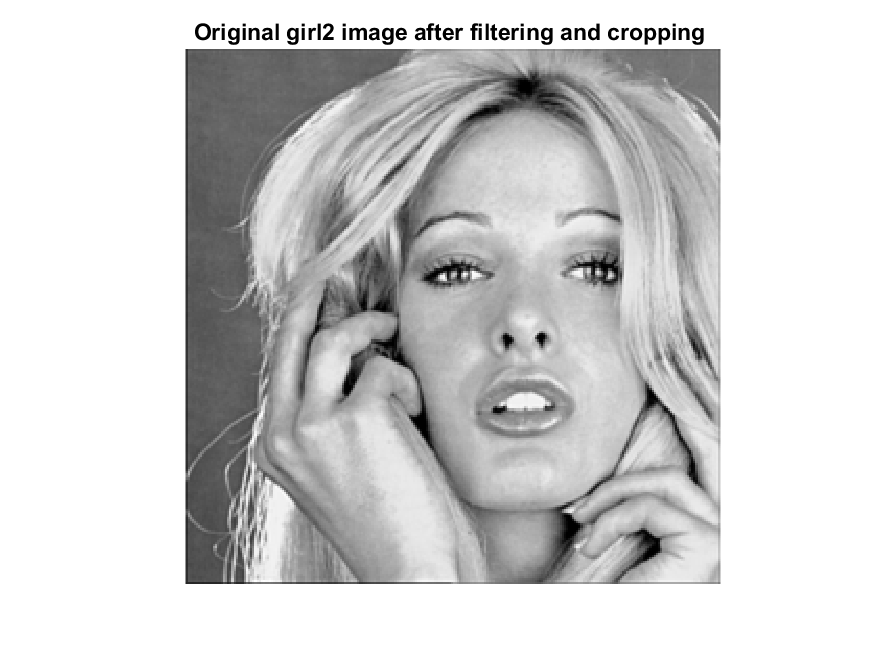
\includegraphics{2cd.png}
\end{figure}
\begin{figure}
 \centering
	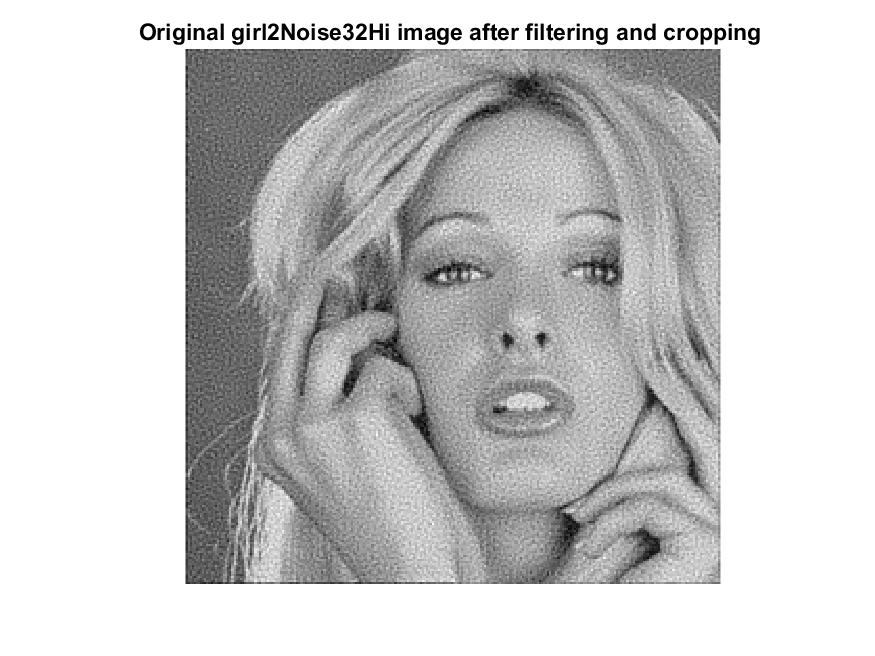
\includegraphics{2ce.png}
	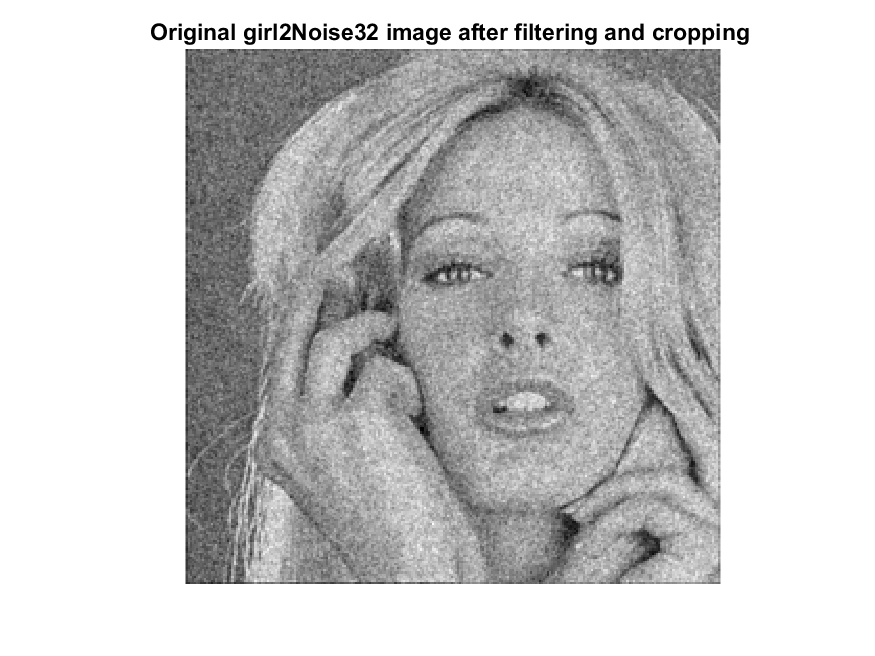
\includegraphics{2cf.png}
\end{figure}
\clearpage

\section {Seventh Answer or 2d}
\subsection*{Matlab Code}
\lstinputlisting{HW5_2d.m}

Output:
\VerbatimInput{Q2d.txt}

Output Images: 
\begin{figure}
 \centering
	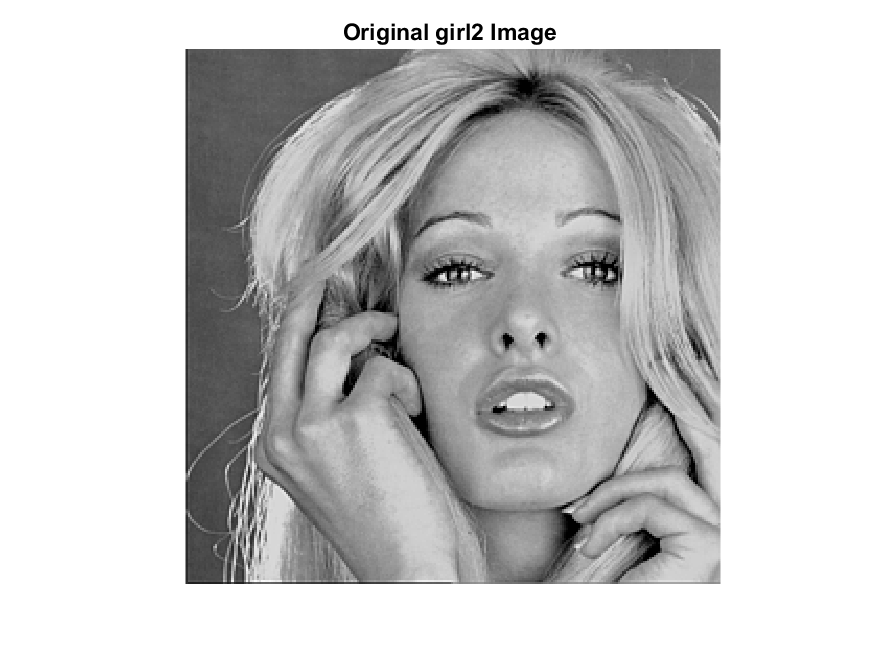
\includegraphics{2da.png}
	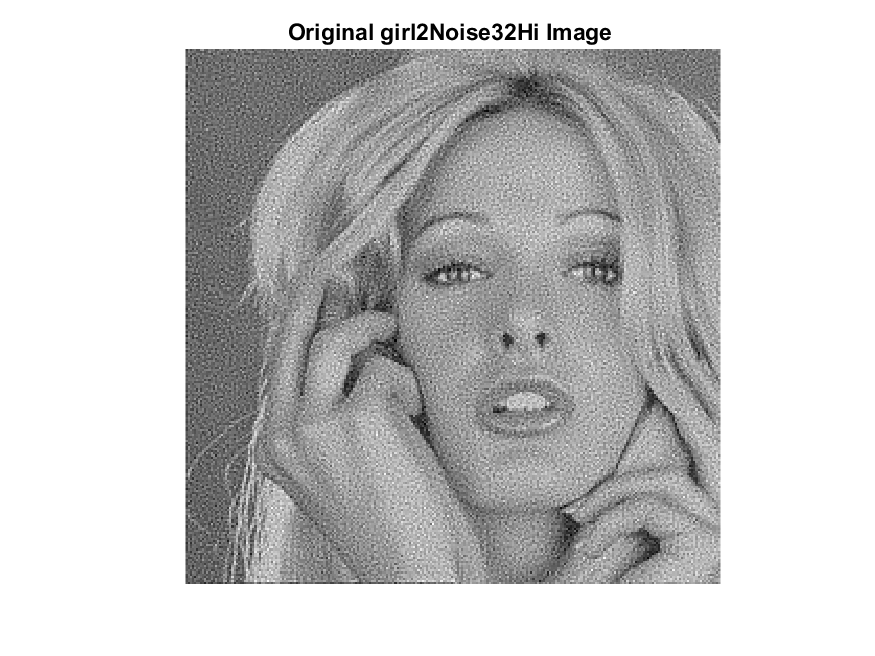
\includegraphics{2db.png}
\end{figure}
\begin{figure}
 \centering
	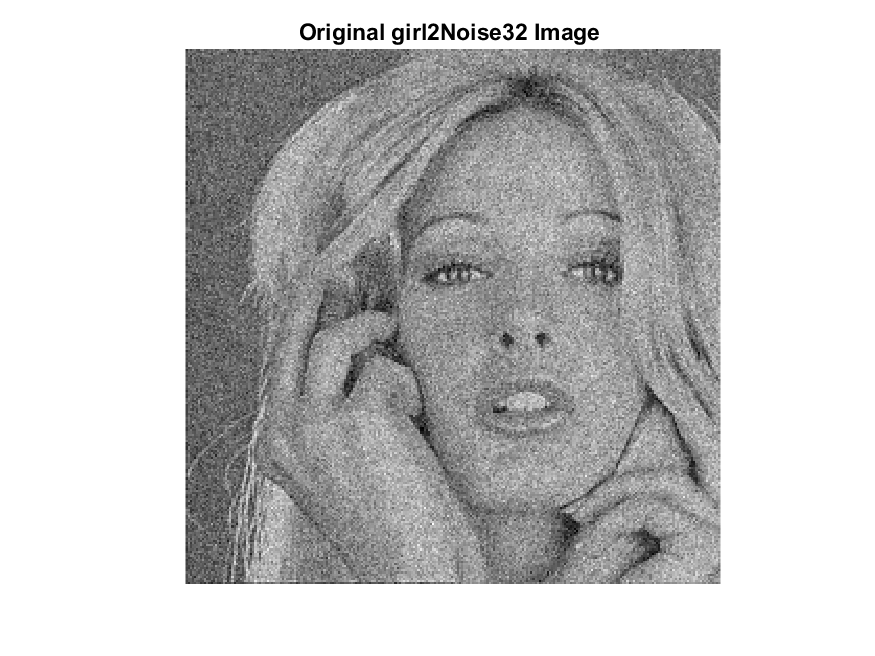
\includegraphics{2dc.png}
	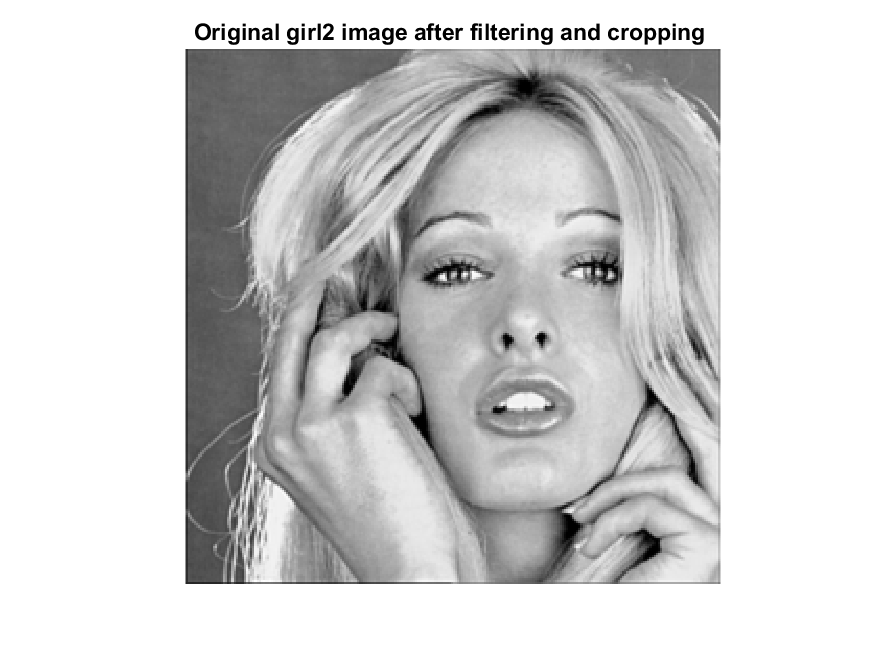
\includegraphics{2dd.png}
\end{figure}
\begin{figure}
 \centering
	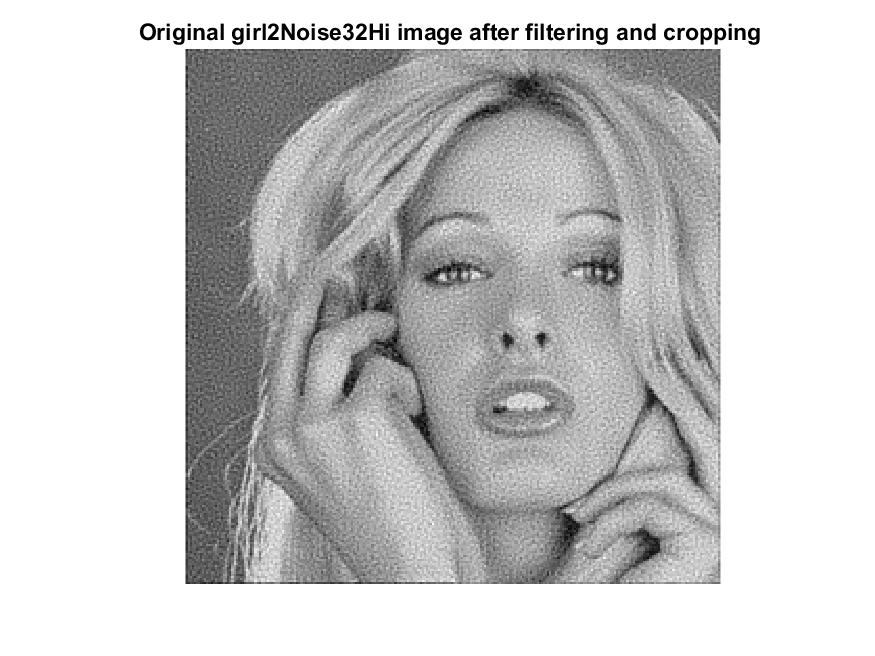
\includegraphics{2de.png}
	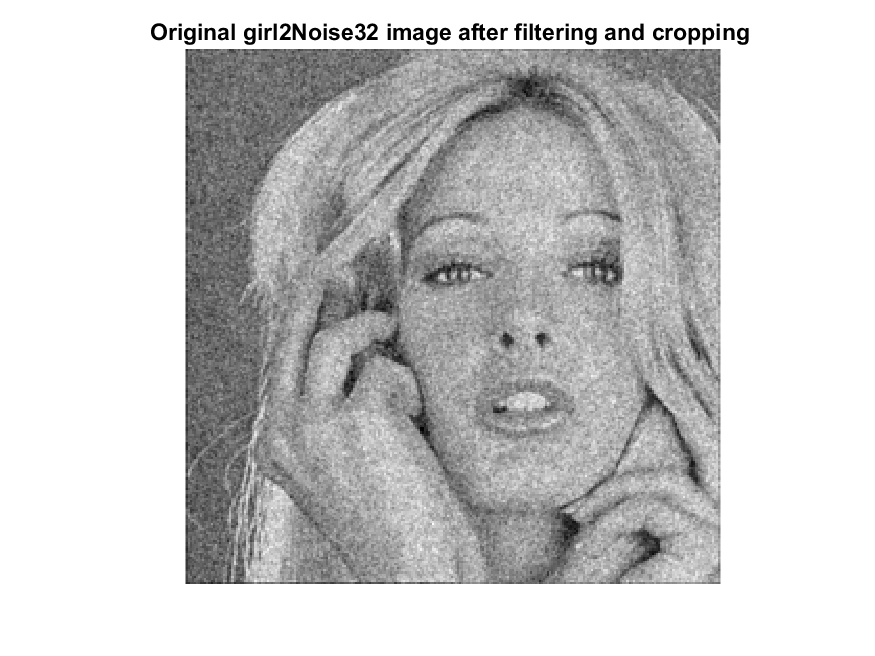
\includegraphics{2df.png}
\end{figure}





\end{document}
